\section{Metodología Experimental}
\label{sec:metodologia}

\subsection{Preguntas de Investigación e Hipótesis de Evaluación}
El diseño experimental responde a tres interrogantes computacionales centrales:
\begin{enumerate}
    \item \textbf{PI1:} ¿Qué estructura de cola de prioridad minimiza el tiempo de pared (\textit{wall-clock time}) en el Algoritmo de Dijkstra sobre redes viales sintéticas dispersas y densas, y cómo evoluciona dicha relación frente al incremento de escala?
    \item \textbf{PI2:} ¿Se traduce la cota asintótica teórica $O(1)$ amortizada en \texttt{Decrease-Key} del Fibonacci Heap en un menor tiempo real de ejecución en un entorno de software interpretado en Python 3.12?
    \item \textbf{PI3:} ¿Qué medianas se observan en la consulta OSM, cuántos vértices expande $A^*$ y cómo cambia el costo estimado con un factor climático uniforme?
\end{enumerate}

\subsubsection{Hipótesis de Trabajo de la Evaluación (H1 a H4)}
\begin{itemize}
    \item \textbf{H1 (Colas en redes dispersas):} En el perfil disperso, el heap binario y el 4-ario podrían registrar menores tiempos que Fibonacci. No se midieron fallos de caché ni asignaciones para atribuirles la diferencia.
    \item \textbf{H2 (Densidad y ramificación):} La diferencia entre 4-ario y binario puede variar con el número de aristas y la escala. El 4-ario tiene menos niveles teóricos, pero compara más hijos al extraer el mínimo.
    \item \textbf{H3 (Poda espacial con búsqueda heurística):} El algoritmo $A^*$ con heurística euclidiana escalada consistente reducirá el número de expansiones de vértices respecto a Dijkstra sin alterar el costo óptimo de la ruta.
    \item \textbf{H4 (Factor uniforme):} Multiplicar por un mismo factor positivo todos los pesos conserva el conjunto de rutas óptimas. Solo se guardó un escenario de sensibilidad climática, no uno de congestión.
\end{itemize}

\subsection{Diseño Factorial e Instancias Experimentales}
El banco canónico de evaluación implementa un diseño factorial completo $3 \times 2 \times 5$:
\begin{itemize}
    \item \textbf{Estructura de cola de prioridad (3 niveles):} Min-Heap Binario Indexado, 4-ary Heap ($d=4$) y Fibonacci Heap.
    \item \textbf{Perfil de densidad del grafo (2 niveles):}
    \begin{itemize}
        \item \textit{Perfil disperso:} $|E| = 4|V|$, parámetro del generador sintético; no es una medición de Cusco.
        \item \textit{Perfil denso:} $|E| \approx 0.08 \, |V|(|V| - 1)$; el generador redondea la cantidad de aristas a un entero.
    \end{itemize}
    \item \textbf{Escala del grafo (5 niveles por perfil):}
    \begin{itemize}
        \item Perfil disperso: $|V| \in \{100, 500, 1000, 2500, 5000\}$.
        \item Perfil denso: $|V| \in \{50, 100, 200, 400, 800\}$.
    \end{itemize}
\end{itemize}

Por escala y perfil se generan tres instancias con semillas fijas. Cada cola se mide 15 veces por instancia, después de dos ejecuciones de calentamiento. Las mediciones repiten los mismos grafos y no son réplicas independientes de redes distintas:
\begin{equation}
    2 \text{ perfiles} \times 5 \text{ escalas} \times 3 \text{ instancias} \times 3 \text{ colas} \times 15 \text{ réplicas} = 1,350 \text{ muestras cronometradas}
    \label{eq:muestras}
\end{equation}

\subsubsection{Generación Determinista de Instancias Sintéticas}
\texttt{benchmark\_network} garantiza alcance desde el origen mediante una cadena dirigida $N_0 \to N_1 \to \dots \to N_{n-1}$; luego agrega aristas aleatorias hasta completar $|E|$. Los pesos provienen de $[1.0,1000.0]$ y son valores sintéticos \emph{sin unidad física}: no representan metros ni segundos de viaje. Con semilla base 12345 y $j\in\{0,1,2\}$ como índice de instancia:
\begin{equation}
    s(n, j) = \begin{cases}
        12345 + 31n + j, & \text{para perfil disperso}, \\
        22345 + 31n + j, & \text{para perfil denso}.
    \end{cases}
    \label{eq:semillas}
\end{equation}

\subsection{Variables Experimentales y Métricas de Desempeño}
\begin{itemize}
    \item \textbf{Variables independientes:} Estructura de cola, escala de vértices $|V|$, densidad de aristas $|E|$ y tipo de grafo (sintético controlado vs. OpenStreetMap real).
    \item \textbf{Variables dependientes:}
    \begin{itemize}
        \item Tiempo de cómputo con reloj de pared, almacenado en microsegundos ($\mu$s) y expresado en milisegundos (ms) cuando se indica.
        \item Estadísticos de tendencia central y dispersión: Mediana e Intervalo Intercuartílico (IQR), seleccionados por su robustez frente a distribuciones asimétricas y ruido del sistema operativo.
        \item Conteo unívoco de primitivas algorítmicas: inserciones (\texttt{Insert}), extracciones (\texttt{Extract-Min}), decrementos efectivos de prioridad (\texttt{Decrease-Key}), intentos totales de relajación y comparaciones de clave ejecutadas.
    \end{itemize}
\end{itemize}

\subsection{Entorno Experimental Controlado e Instrumentación de Precisión}
El banco guardado registra Python y plataforma. La Tabla~\ref{tab:entorno} describe el equipo de trabajo usado; no se midió ni controló la carga del sistema o la jerarquía de caché durante cada ejecución.

\begin{table}[H]
    \centering
    \fontsize{9.5}{11.5}\selectfont
    \caption{Especificaciones del entorno experimental de medición}
    \label{tab:entorno}
    \begin{tabular}{@{}ll@{}}
        \toprule
        \textbf{Componente / Parámetro} & \textbf{Especificación Técnica} \\
        \midrule
        Sistema Operativo & Microsoft Windows 11 Pro 64-bit (Build 10.0.26300) \\
        Procesador (CPU) & AMD Ryzen 5 5600H @ 3.30 GHz (Turbo hasta 4.2 GHz) \\
        Configuración de núcleos & 6 núcleos físicos, 12 subprocesos lógicos \\
        Jerarquía de Caché & L1: 384 KB, L2: 3 MB, L3: 16 MB compartida \\
        Memoria RAM & 24 GB DDR4 @ 3200 MHz \\
        Plataforma de Software & Python 3.12.8 (64-bit) \\
        Frameworks Auxiliares & pytest 9.1.1, NetworkX 3.7, OSMnx 2.1.1 \\
        \bottomrule
    \end{tabular}
\end{table}

\subsubsection{Protocolo de Aislamiento de Ruido y Precisión Temporal}
\begin{enumerate}
    \item \textbf{Temporizador:} Se usa \texttt{time.perf\_counter\_ns()} y se convierten los intervalos medidos a microsegundos. El nombre del reloj no implica una precisión efectiva de un nanosegundo.
    \item \textbf{Recolector de basura:} Antes de cada muestra se invoca \texttt{gc.collect()} y se desactiva el recolector automático durante la llamada cronometrada; al terminar se restaura su estado anterior.
    \item \textbf{Calentamiento:} Se descartan dos ejecuciones previas por combinación de instancia y cola; no se midió su efecto sobre la frecuencia del procesador ni sobre las cachés.
    \item \textbf{Orden de colas:} Para cada instancia se permuta de forma reproducible el orden de las tres colas para reducir un posible sesgo de orden. Esto no elimina el ruido del sistema.
    \item \textbf{Verificación previa:} Antes de medir cada instancia sintética se comparan las distancias de las tres colas, se contrastan con NetworkX y se certifica una solución. Bellman-Ford se contrasta por separado en la suite de pruebas.
\end{enumerate}

\subsection{Caso Aplicado sobre la Red Vial Urbana Real de Cusco}
Para evaluar el comportamiento de los algoritmos en una red urbana real, se extrajo la malla vial del Centro y áreas adyacentes de la ciudad del Cusco mediante OSMnx 2.1.1 a partir de las coordenadas $(-13.5165, -71.9788)$ con un radio de 1.5 km en modalidad \texttt{drive}. La red comprende 891 intersecciones y 2,139 tramos dirigidos ($|E|/|V| = 2.40$).

El par se seleccionó con una regla fija: el origen $s$ es el nodo más cercano al centro de extracción y el destino $t$ es el nodo alcanzable de mayor costo temporal base. La misma consulta se midió 30 veces por cola, con tres calentamientos previos; no se muestrearon pares de rutas independientes. Para $A^*$ se usó una heurística euclidiana escalada consistente:
\begin{equation}
    h(u) = \lambda \cdot \|x_u - x_t\|, \quad \text{donde } \lambda = \min_{(u, v) \in E} \frac{w(u, v)}{\|x_u - x_v\|}
    \label{eq:heuristica_escalada}
\end{equation}
y se analizó la sensibilidad del trayecto bajo el factor meteorológico compuesto de Open-Meteo ($m_{\text{clima}} = 1.0691$).

\subsection{Procedimiento Experimental Reproducible}
El script siguiente conserva separadas la medición y la generación de tablas y figuras. Los tiempos guardados están en microsegundos; las tablas de la consulta OSM los expresan en milisegundos. El tiempo de viaje calculado para la ruta está en segundos y no mide la ejecución del programa.
\begin{lstlisting}[language=bash, caption={Comando de reproducción de figuras y tablas científicas}]
# Regeneración sin repetir mediciones (reutiliza los 1350 datos guardados en JSON):
python python/scripts/reproduce_canonical.py --skip-benchmark --skip-applied

# Ejecución completa del benchmark canónico (1350 corridas):
python python/scripts/reproduce_canonical.py
\end{lstlisting}

\subsection{Piloto de Verificación del Protocolo}
El piloto guardado el 04/11/2026 verificó el protocolo en dos grafos de 100 vértices: uno disperso (400 aristas) y uno denso (792). Se usó una instancia por perfil, tres colas y tres mediciones por cola, con dos calentamientos previos: 18 muestras cronometradas. El script comprobó las distancias frente a NetworkX y el certificado antes de medir. \texttt{python/data/processed/pilot\_benchmark\_results.json} conserva muestras, semillas y estadísticos; la Figura~\ref{fig:piloto_mediciones} muestra esas muestras. El piloto se hizo \emph{después} del banco canónico fechado el 28/10/2026: comprueba que el procedimiento se puede repetir, pero sus tres mediciones por cola no bastan para decidir qué cola rinde mejor. La semilla reproduce los grafos, no el tiempo de reloj. Desde la raíz del repositorio:
\begin{lstlisting}[language=bash, caption={Reproducción del ensayo piloto y su figura}]
python python/scripts/reproduce_pilot.py
# Solo regenerar la figura sin repetir mediciones:
python python/scripts/reproduce_pilot.py --plot-only
\end{lstlisting}

\begin{figure}[H]
    \centering
    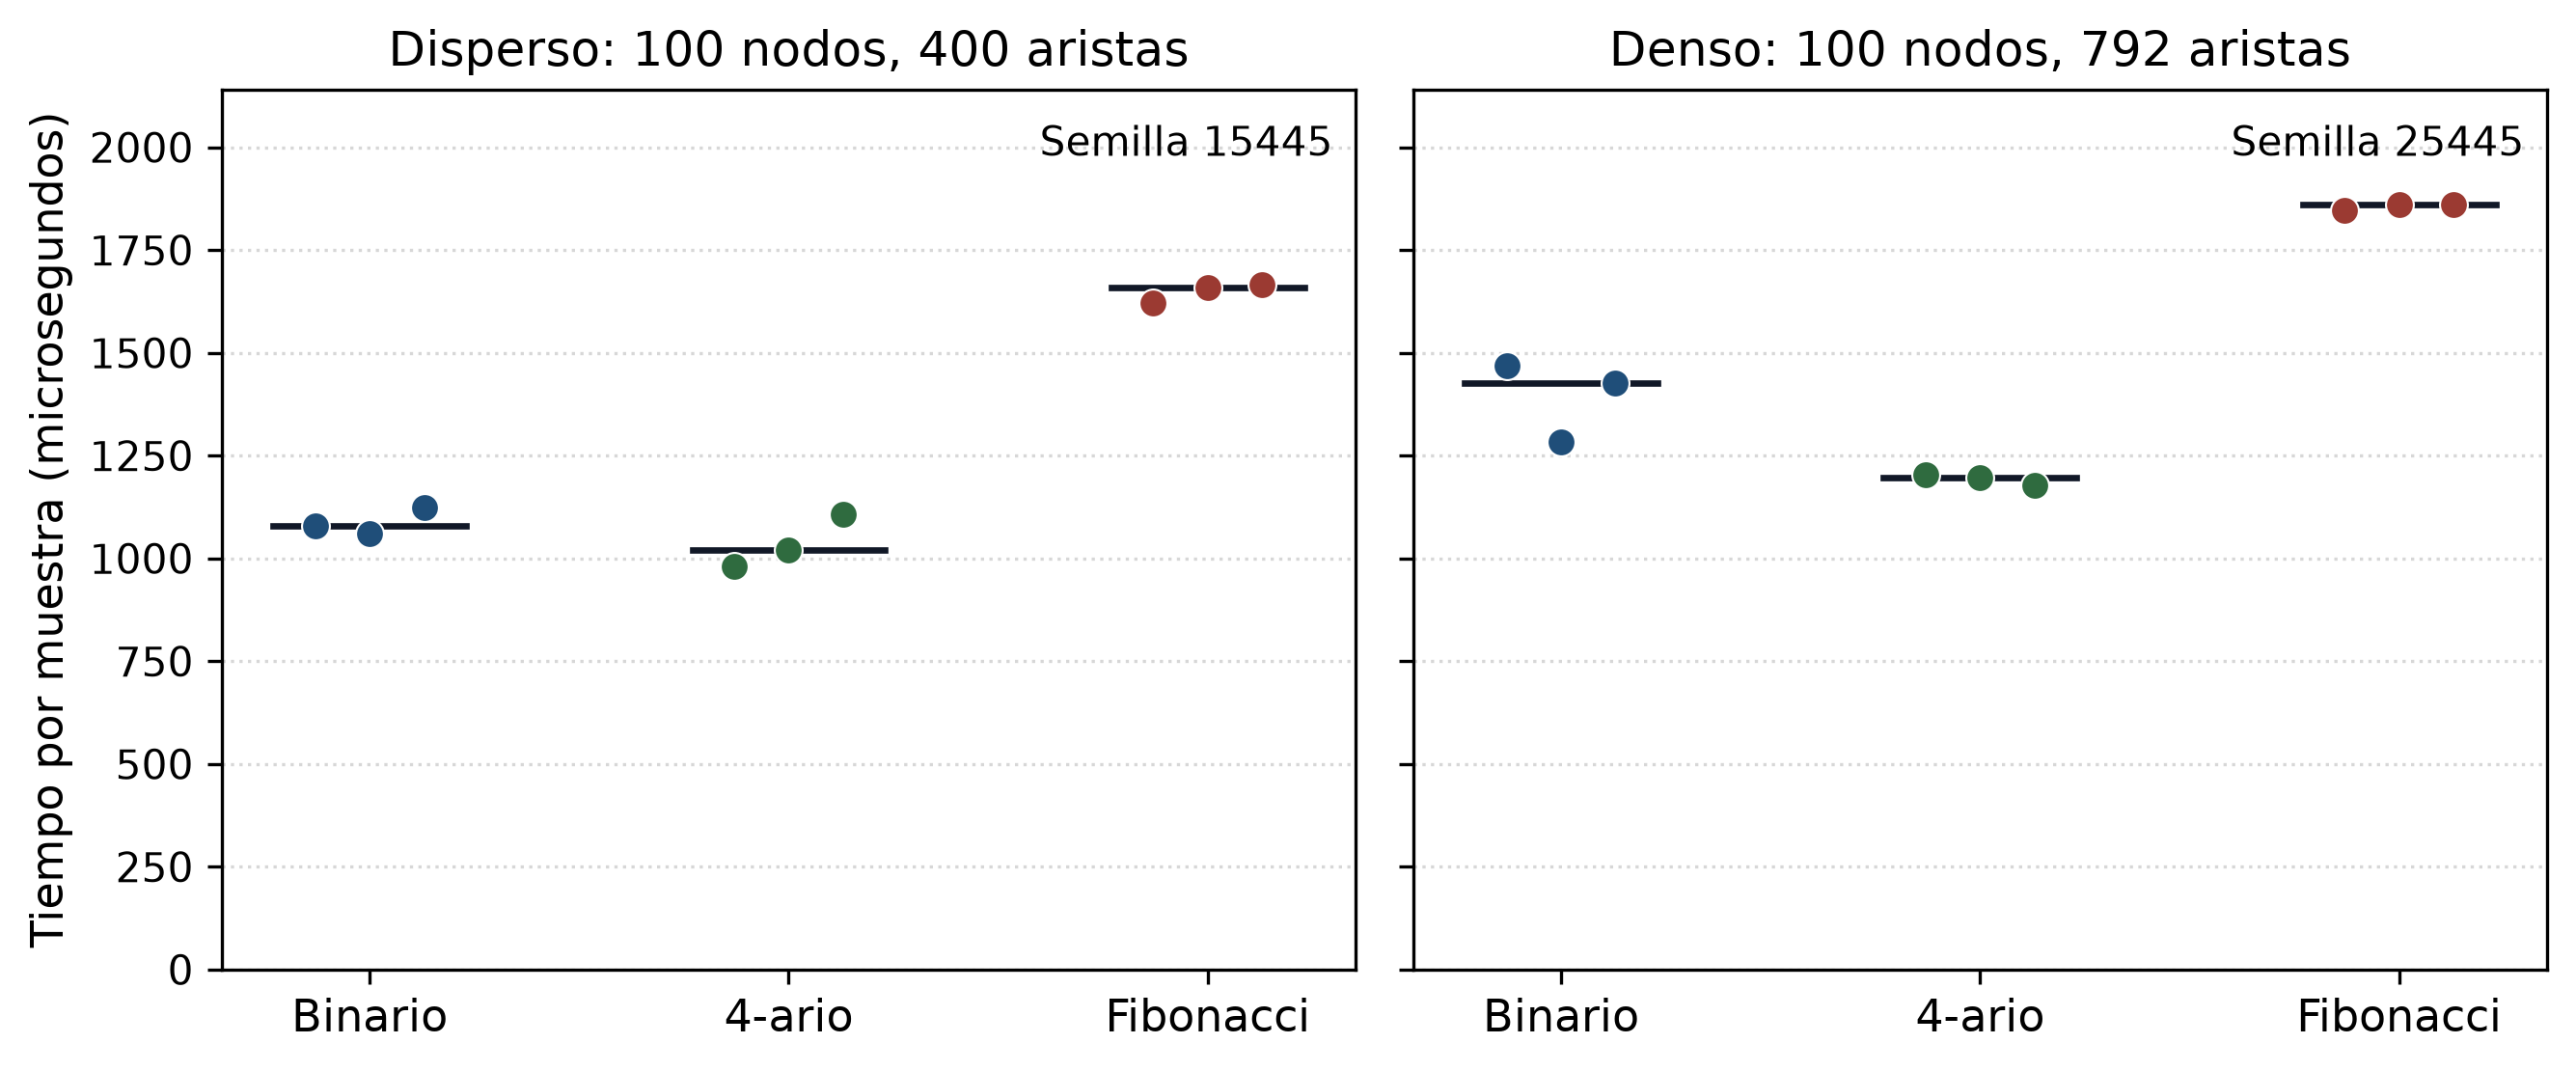
\includegraphics[width=\textwidth]{figuras/piloto_mediciones.png}
    \caption{Piloto del 04/11/2026. Cada punto representa una medición; el segmento, la mediana de tres repeticiones. Datos: \texttt{pilot\_benchmark\_results.json}. La comparación por escenario se presenta en la Sección~\ref{sec:resultados}.}
    \label{fig:piloto_mediciones}
\end{figure}

\subsection{Amenazas a la Validez}
\begin{itemize}
    \item \textbf{Validez interna:} El planificador y la frecuencia del procesador pueden alterar los tiempos. El calentamiento y la desactivación del GC reducen algunas fuentes de variación, pero no las eliminan. Mediana e IQR describen las muestras; no corrigen el ruido.
    \item \textbf{Validez externa:} Las mediciones proceden de Python 3.12 en un procesador AMD Ryzen. No se puede extrapolar la diferencia observada a otros lenguajes o equipos sin repetir el experimento.
    \item \textbf{Validez de conclusión:} El solapamiento de IQR describe dispersión, pero por sí solo no es una prueba de significación estadística ni de igualdad entre colas. No se midieron contadores físicos de caché ni consumo de memoria.
\end{itemize}
